\documentclass[a4paper, 10pt]{article}
\usepackage[utf8]{inputenc}
\usepackage[T1]{fontenc}
\usepackage[spanish]{babel}
\usepackage{lmodern}
\usepackage{amsmath, amssymb}
\usepackage[margin=1.0cm, top=0.8cm, bottom=0.8cm]{geometry}
\usepackage{graphicx}
\graphicspath{{../Figures/}{Figures/}}
\usepackage{tikz}
\usetikzlibrary{arrows.meta, calc, positioning, decorations.pathreplacing, shapes}
\usepackage{tcolorbox}
\tcbuselibrary{skins}
\usepackage{enumitem}
\usepackage[dvipsnames]{xcolor}
\usepackage{siunitx}

\sisetup{
    output-decimal-marker = {,},
    separate-uncertainty  = true,
    per-mode              = symbol,
}

\pagestyle{empty}

\definecolor{uni-blue}{RGB}{0, 56, 101}
\definecolor{uni-red}{RGB}{166, 25, 46}
\definecolor{box-green}{RGB}{24, 134, 75}
\definecolor{box-purple}{RGB}{112, 48, 160}

%% Macro limpia para figura centrada en 1 columna con marco discontinuo de recorte
\newcommand{\stickersingle}[2]{%
    \begin{center}
        {\footnotesize\bfseries\color{uni-blue} #1}\\[1.2mm]
        \begin{tikzpicture}
            \node[draw=gray!60, dashed, line width=0.5pt, inner sep=1.2mm, fill=white] {
                #2
            };
        \end{tikzpicture}
    \end{center}%
}

\begin{document}

%% ============================================================
%% PÁGINA 1: JESÚS VERA (PORTADA Y MATERIALES)
%% ============================================================
\noindent
\begin{minipage}{\linewidth}
    \centering
    {\large\bfseries\color{uni-blue} GUÍA DE FIGURAS Y GRÁFICAS PARA IMPRESIÓN (STICKERS / RECORTES)}\\[0.5mm]
    {\footnotesize\textbf{Página 1 de 5: Portada y Sección 5 --- Materiales y Equipos (Jesús Vera)}}\\[0.8mm]
    \hrule height 0.8pt
\end{minipage}

\vspace{3mm}

\stickersingle{Escudo Oficial UNI (Portada)}{%
    
\includegraphics[width=3.6cm, height=4.5cm, keepaspectratio=true]{uni_logo.jpg}%
}

\vspace{2mm}

%% Fila 1: Fuente DC y Multímetro
\noindent
\begin{minipage}[t]{0.48\linewidth}
    \centering
    {\footnotesize\bfseries\color{uni-blue} Figura 1: Fuente DC Regulada (0--30 V)}\\[1.2mm]
    \begin{tikzpicture}
        \node[draw=gray!60, dashed, line width=0.5pt, inner sep=1.2mm, fill=white] {
            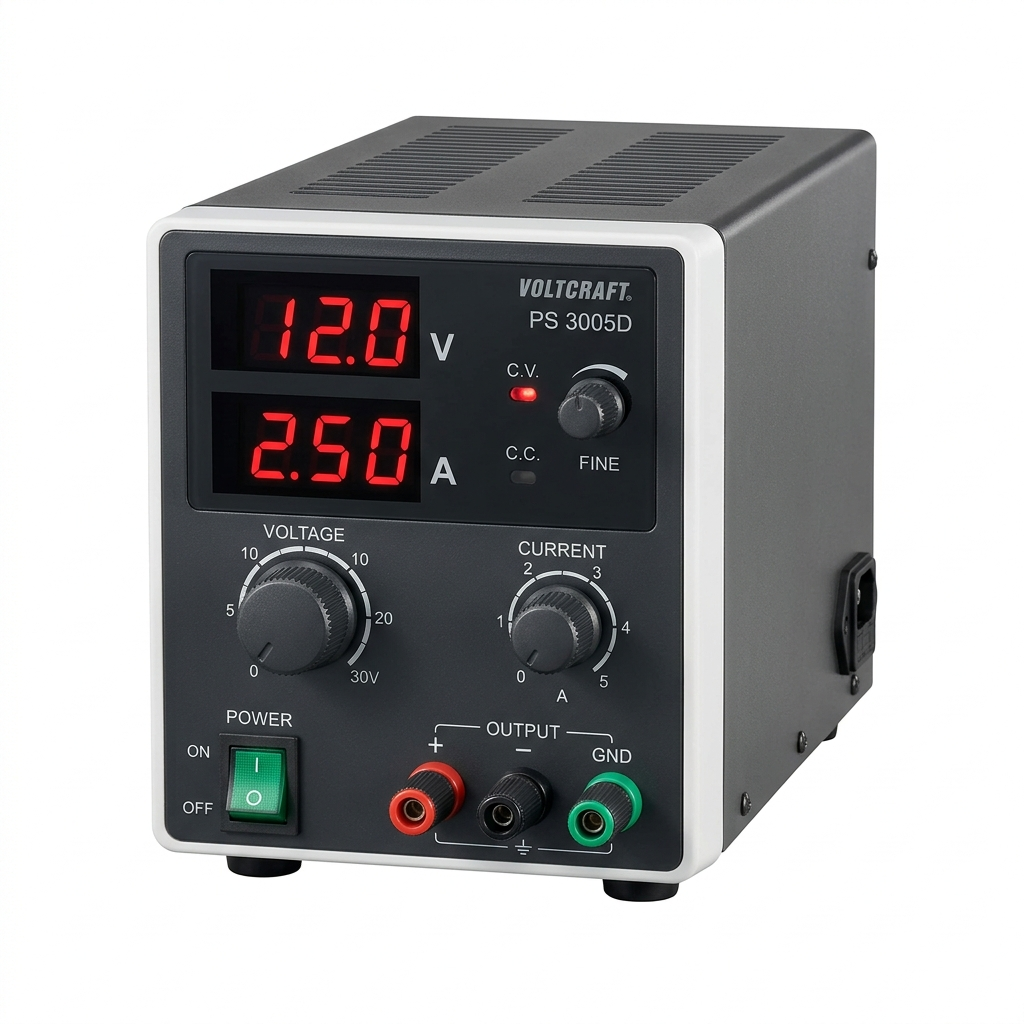
\includegraphics[width=6.2cm, height=4.8cm, keepaspectratio=true]{fig_fuente_dc.png}
        };
    \end{tikzpicture}
\end{minipage}%
\hfill
\begin{minipage}[t]{0.48\linewidth}
    \centering
    {\footnotesize\bfseries\color{uni-blue} Figura 2: Multímetro Digital de Precisión}\\[1.2mm]
    \begin{tikzpicture}
        \node[draw=gray!60, dashed, line width=0.5pt, inner sep=1.2mm, fill=white] {
            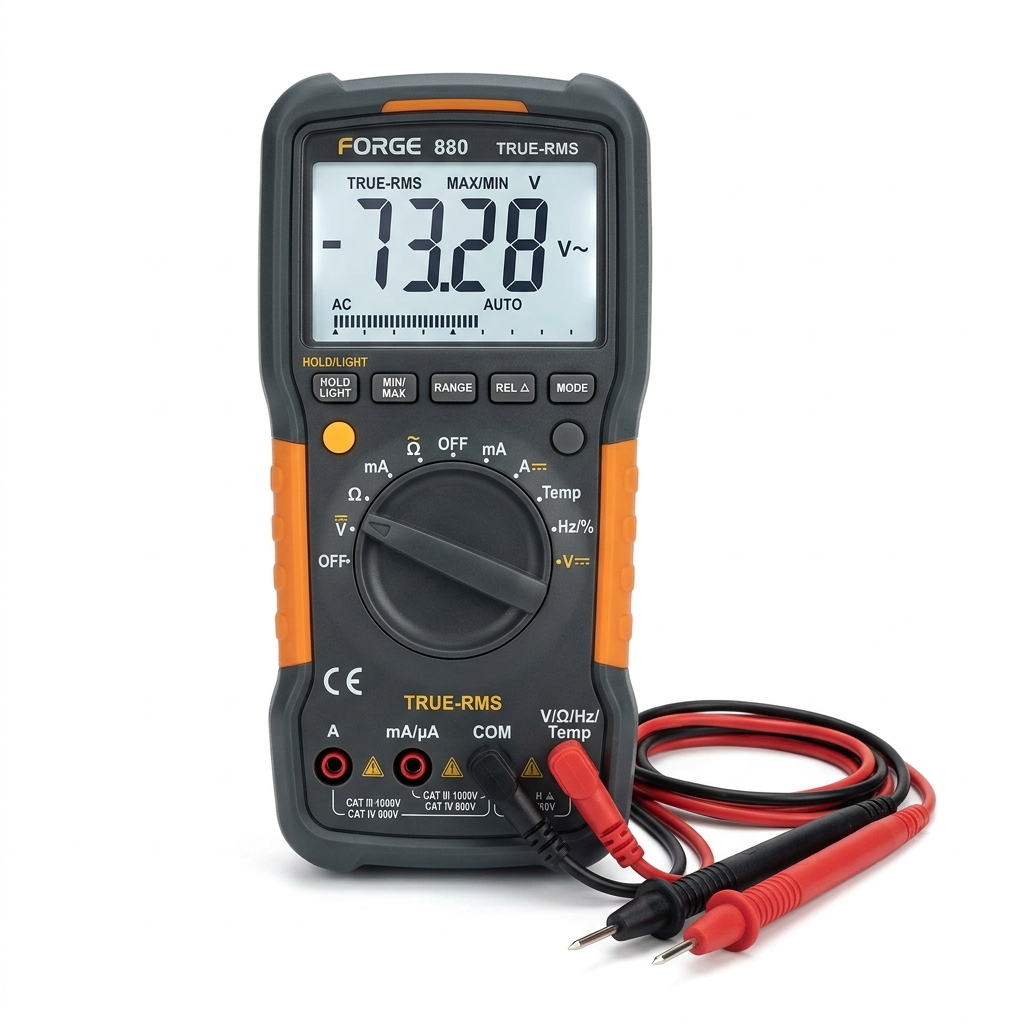
\includegraphics[width=6.2cm, height=4.8cm, keepaspectratio=true]{fig_multimetro.png}
        };
    \end{tikzpicture}
\end{minipage}

\vspace{3mm}

%% Fila 2: Reóstato y Caja de Elementos
\noindent
\begin{minipage}[t]{0.48\linewidth}
    \centering
    {\footnotesize\bfseries\color{uni-blue} Figura 3: Reóstato / Potenciómetro de Laboratorio}\\[1.2mm]
    \begin{tikzpicture}
        \node[draw=gray!60, dashed, line width=0.5pt, inner sep=1.2mm, fill=white] {
            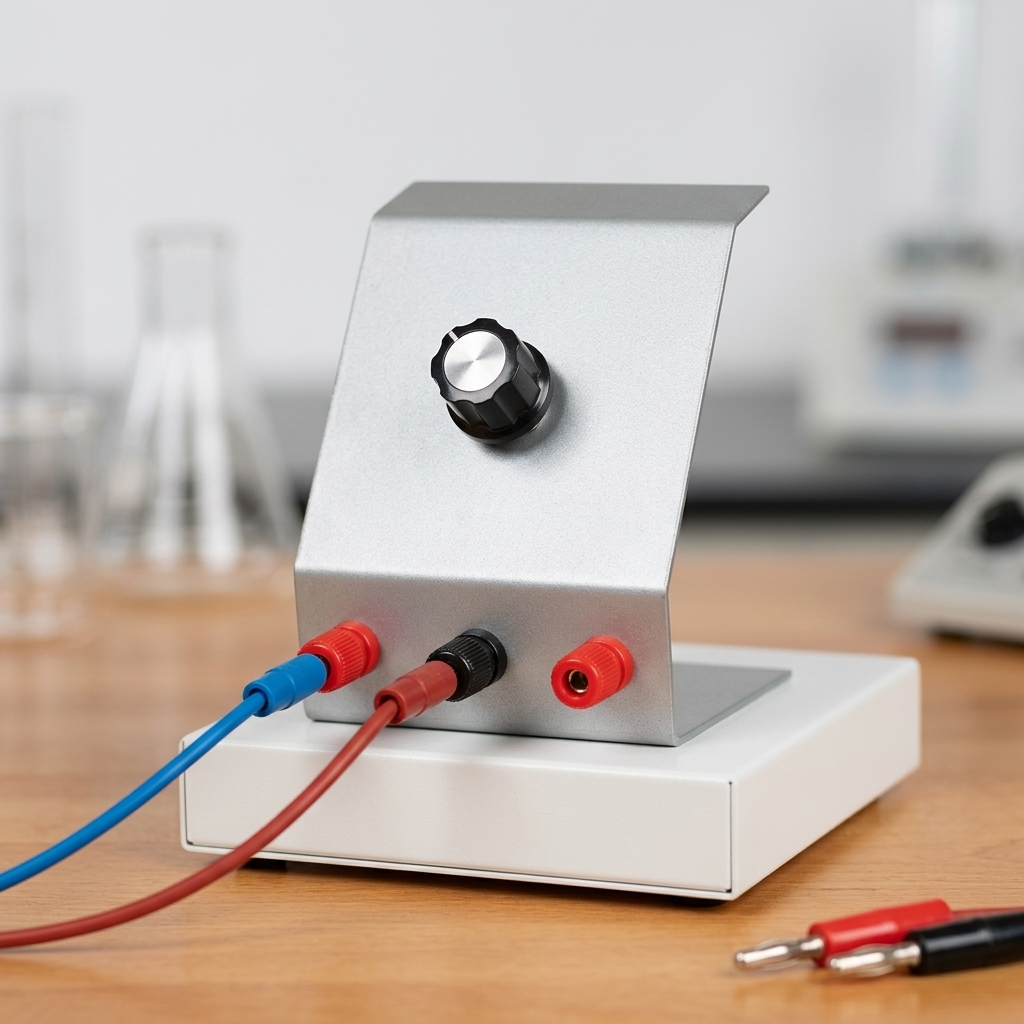
\includegraphics[width=6.2cm, height=4.8cm, keepaspectratio=true]{fig_reostato.png}
        };
    \end{tikzpicture}
\end{minipage}%
\hfill
\begin{minipage}[t]{0.48\linewidth}
    \centering
    {\footnotesize\bfseries\color{uni-blue} Figura 4: Caja de Elementos de Prueba}\\[1.2mm]
    \begin{tikzpicture}
        \node[draw=gray!60, dashed, line width=0.5pt, inner sep=1.2mm, fill=white] {
            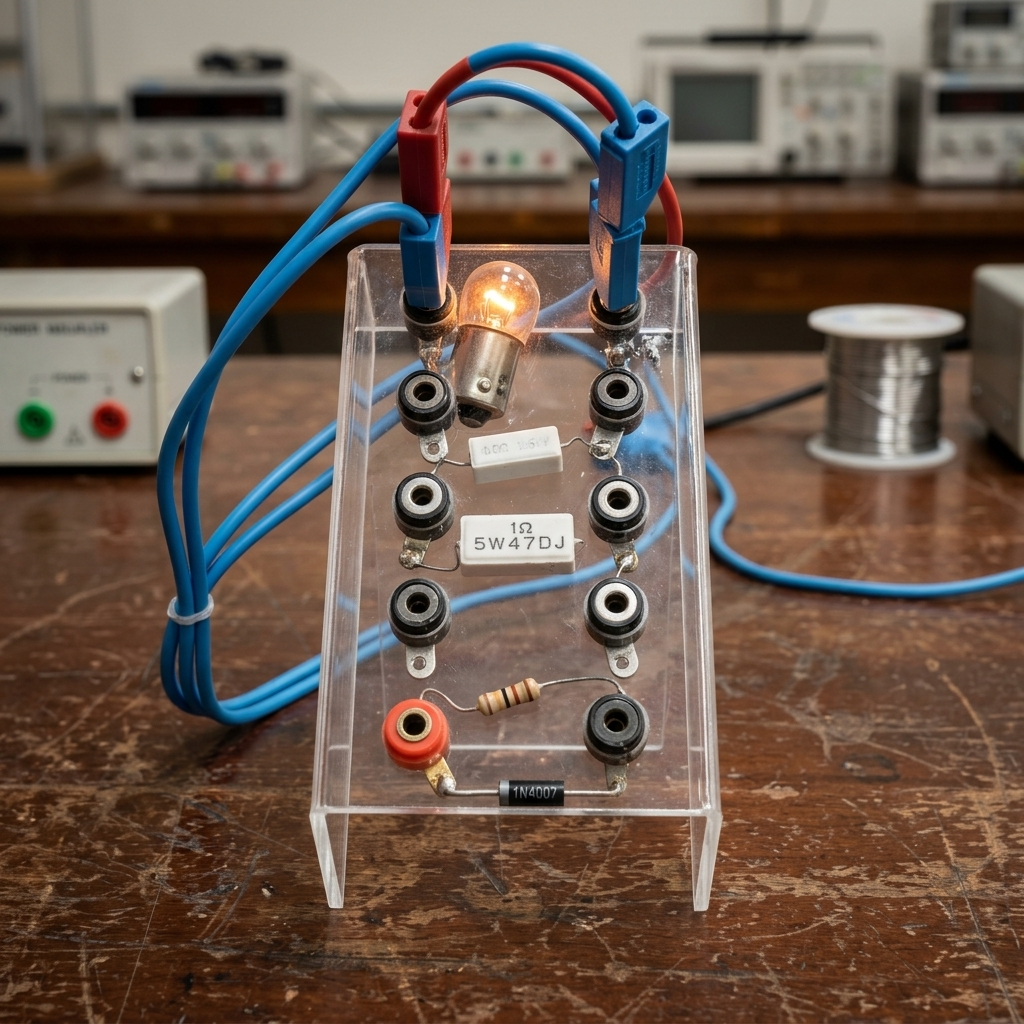
\includegraphics[width=6.2cm, height=4.8cm, keepaspectratio=true]{fig_caja_elementos.png}
        };
    \end{tikzpicture}
\end{minipage}

\vspace{3mm}

%% Fila 3: Cables y Terminales
\noindent
\begin{center}
    {\footnotesize\bfseries\color{uni-blue} Figura 5: Cables Conductores y Terminales Banana--Caimán}\\[1.2mm]
    \begin{tikzpicture}
        \node[draw=gray!60, dashed, line width=0.5pt, inner sep=1.2mm, fill=white] {
            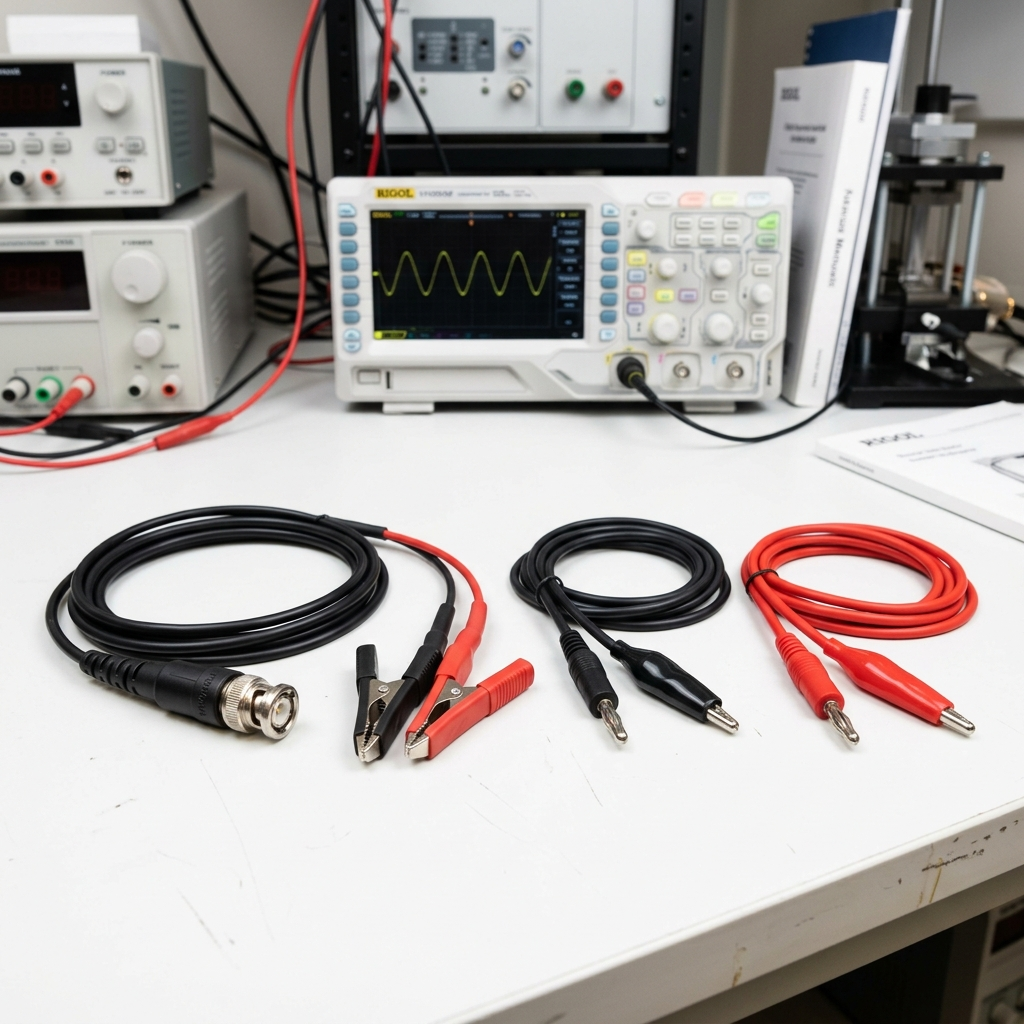
\includegraphics[width=6.8cm, height=4.5cm, keepaspectratio=true]{fig_cables_sondas.jpg}
        };
    \end{tikzpicture}
\end{center}

\newpage

%% ============================================================
%% PÁGINA 2: GERALD CASAÑE (PROCEDIMIENTO EXPERIMENTAL Y MONTAJE)
%% ============================================================
\noindent
\begin{minipage}{\linewidth}
    \centering
    {\large\bfseries\color{uni-blue} GUÍA DE FIGURAS Y GRÁFICAS PARA IMPRESIÓN (STICKERS / RECORTES)}\\[0.5mm]
    {\footnotesize\textbf{Página 2 de 5: Sección 6 --- Montaje Circuital y Procedimiento (Gerald Casañe)}}\\[0.8mm]
    \hrule height 0.8pt
\end{minipage}

\vspace{4mm}

\stickersingle{Figura 6: Esquema Circuital del Divisor de Voltaje con Reóstato y Carga bajo Ensayo}{%
    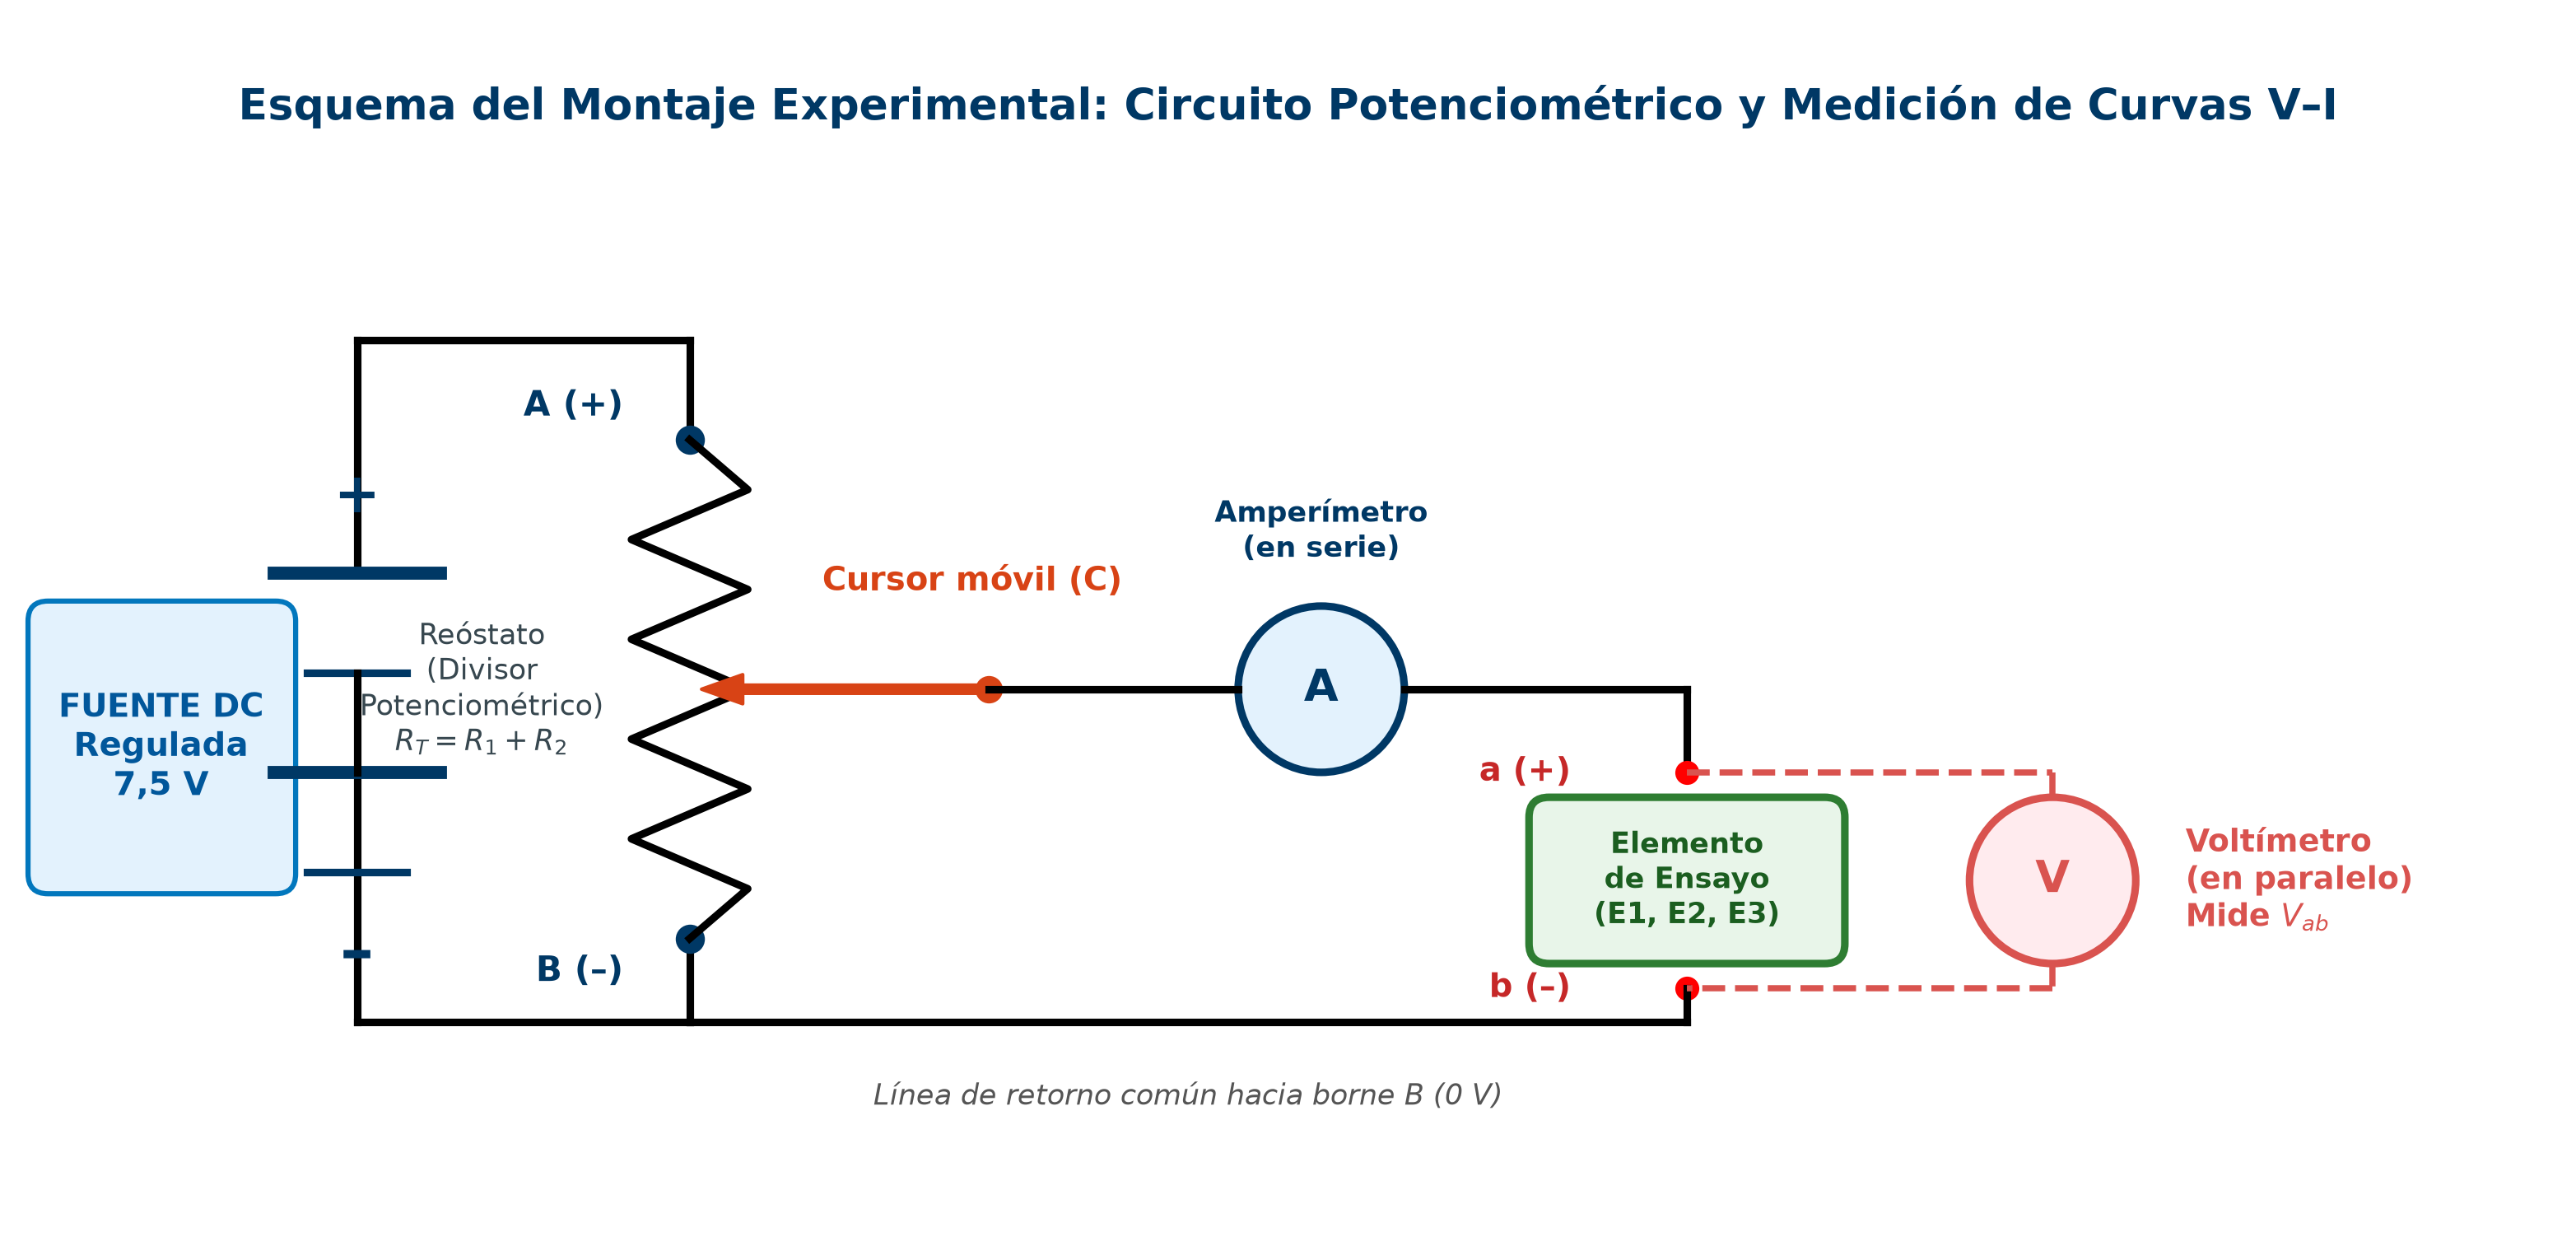
\includegraphics[width=14.5cm, height=6.2cm, keepaspectratio=true]{fig_circuito_potenciometro.png}%
}

\vspace{5mm}

\noindent
\begin{tcolorbox}[sharp corners, boxrule=0.6pt, colback=gray!5, colframe=uni-blue, center, width=0.96\linewidth]
    \footnotesize
    \textbf{Instrucciones de Montaje para Gerald Casañe (Bloque 2):}
    \begin{itemize}[leftmargin=1.2em, itemsep=2.5pt]
        \item Pegar la \textbf{Figura 6} centrada en la Sección 6 (Procedimiento Experimental) antes de detallar los pasos secuenciales de las Partes A, B, C y D.
        \item Trazar las \textbf{Tablas 2, 3, 4 y 5} de Resultados con regla milimetrada respetando el formato formal (solo 3 líneas horizontales tipo \textit{booktabs}, sin líneas verticales divisorias).
        \item Desarrollar paso a paso las fórmulas algebraicas de los mínimos cuadrados (MCO) de la resistencia de carbón, la regresión logarítmica del foquito, el ajuste de Shockley del diodo y la deducción teórica de radiación térmica de Stefan-Boltzmann en el \textbf{Anexo A}.
    \end{itemize}
\end{tcolorbox}

\newpage

%% ============================================================
%% PÁGINA 3: PIERO SÁNCHEZ (GRÁFICAS CIENTÍFICAS PYTHON 1 Y 2)
%% ============================================================
\noindent
\begin{minipage}{\linewidth}
    \centering
    {\large\bfseries\color{uni-blue} GUÍA DE FIGURAS Y GRÁFICAS PARA IMPRESIÓN (STICKERS / RECORTES)}\\[0.5mm]
    {\footnotesize\textbf{Página 3 de 5: Sección 10 --- Resistencia de Carbón y Foquito (Piero Sánchez)}}\\[0.8mm]
    \hrule height 0.8pt
\end{minipage}

\vspace{3mm}

\stickersingle{Figura 7: Curva Característica $I$ vs $V$ de la Resistencia de Carbón ($100\,\Omega$)}{%
    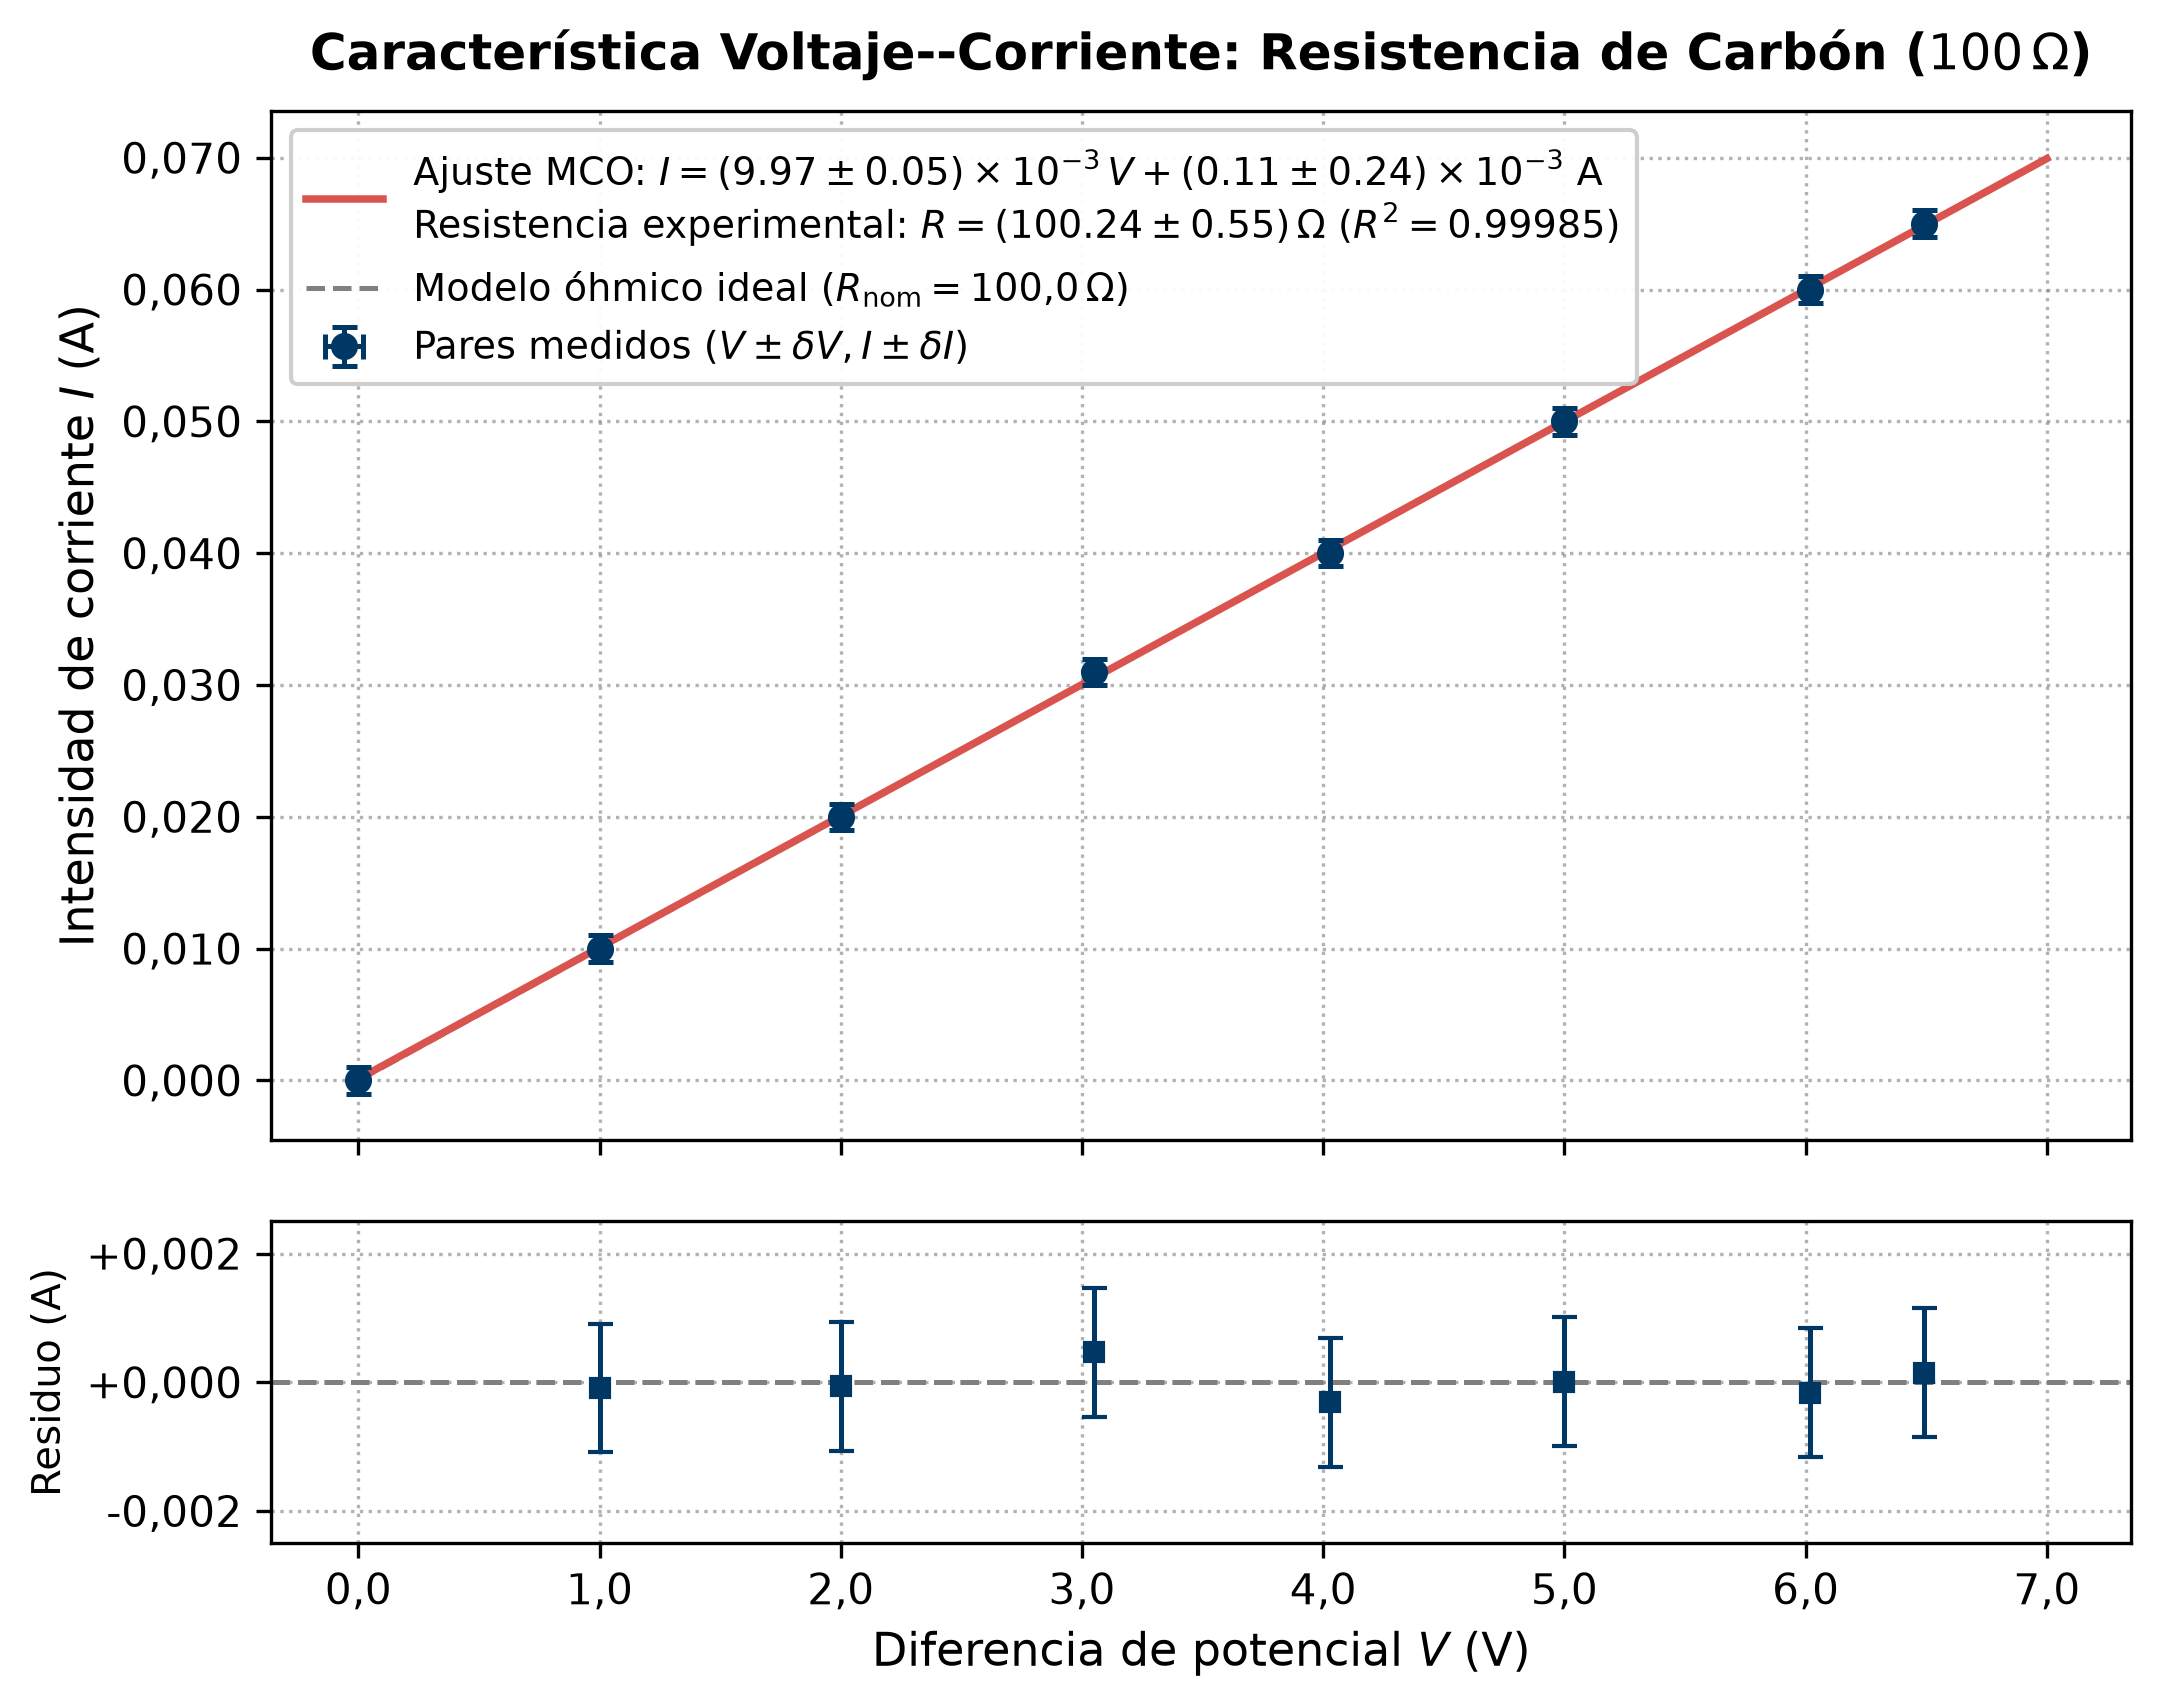
\includegraphics[width=14.0cm, height=9.0cm, keepaspectratio=true]{fig_resistencia_ohmica.png}%
}

\vspace{4mm}

\stickersingle{Figura 8: Curva Característica $I$ vs $V$ de la Lámpara de Tungsteno y Ajuste de Potencia}{%
    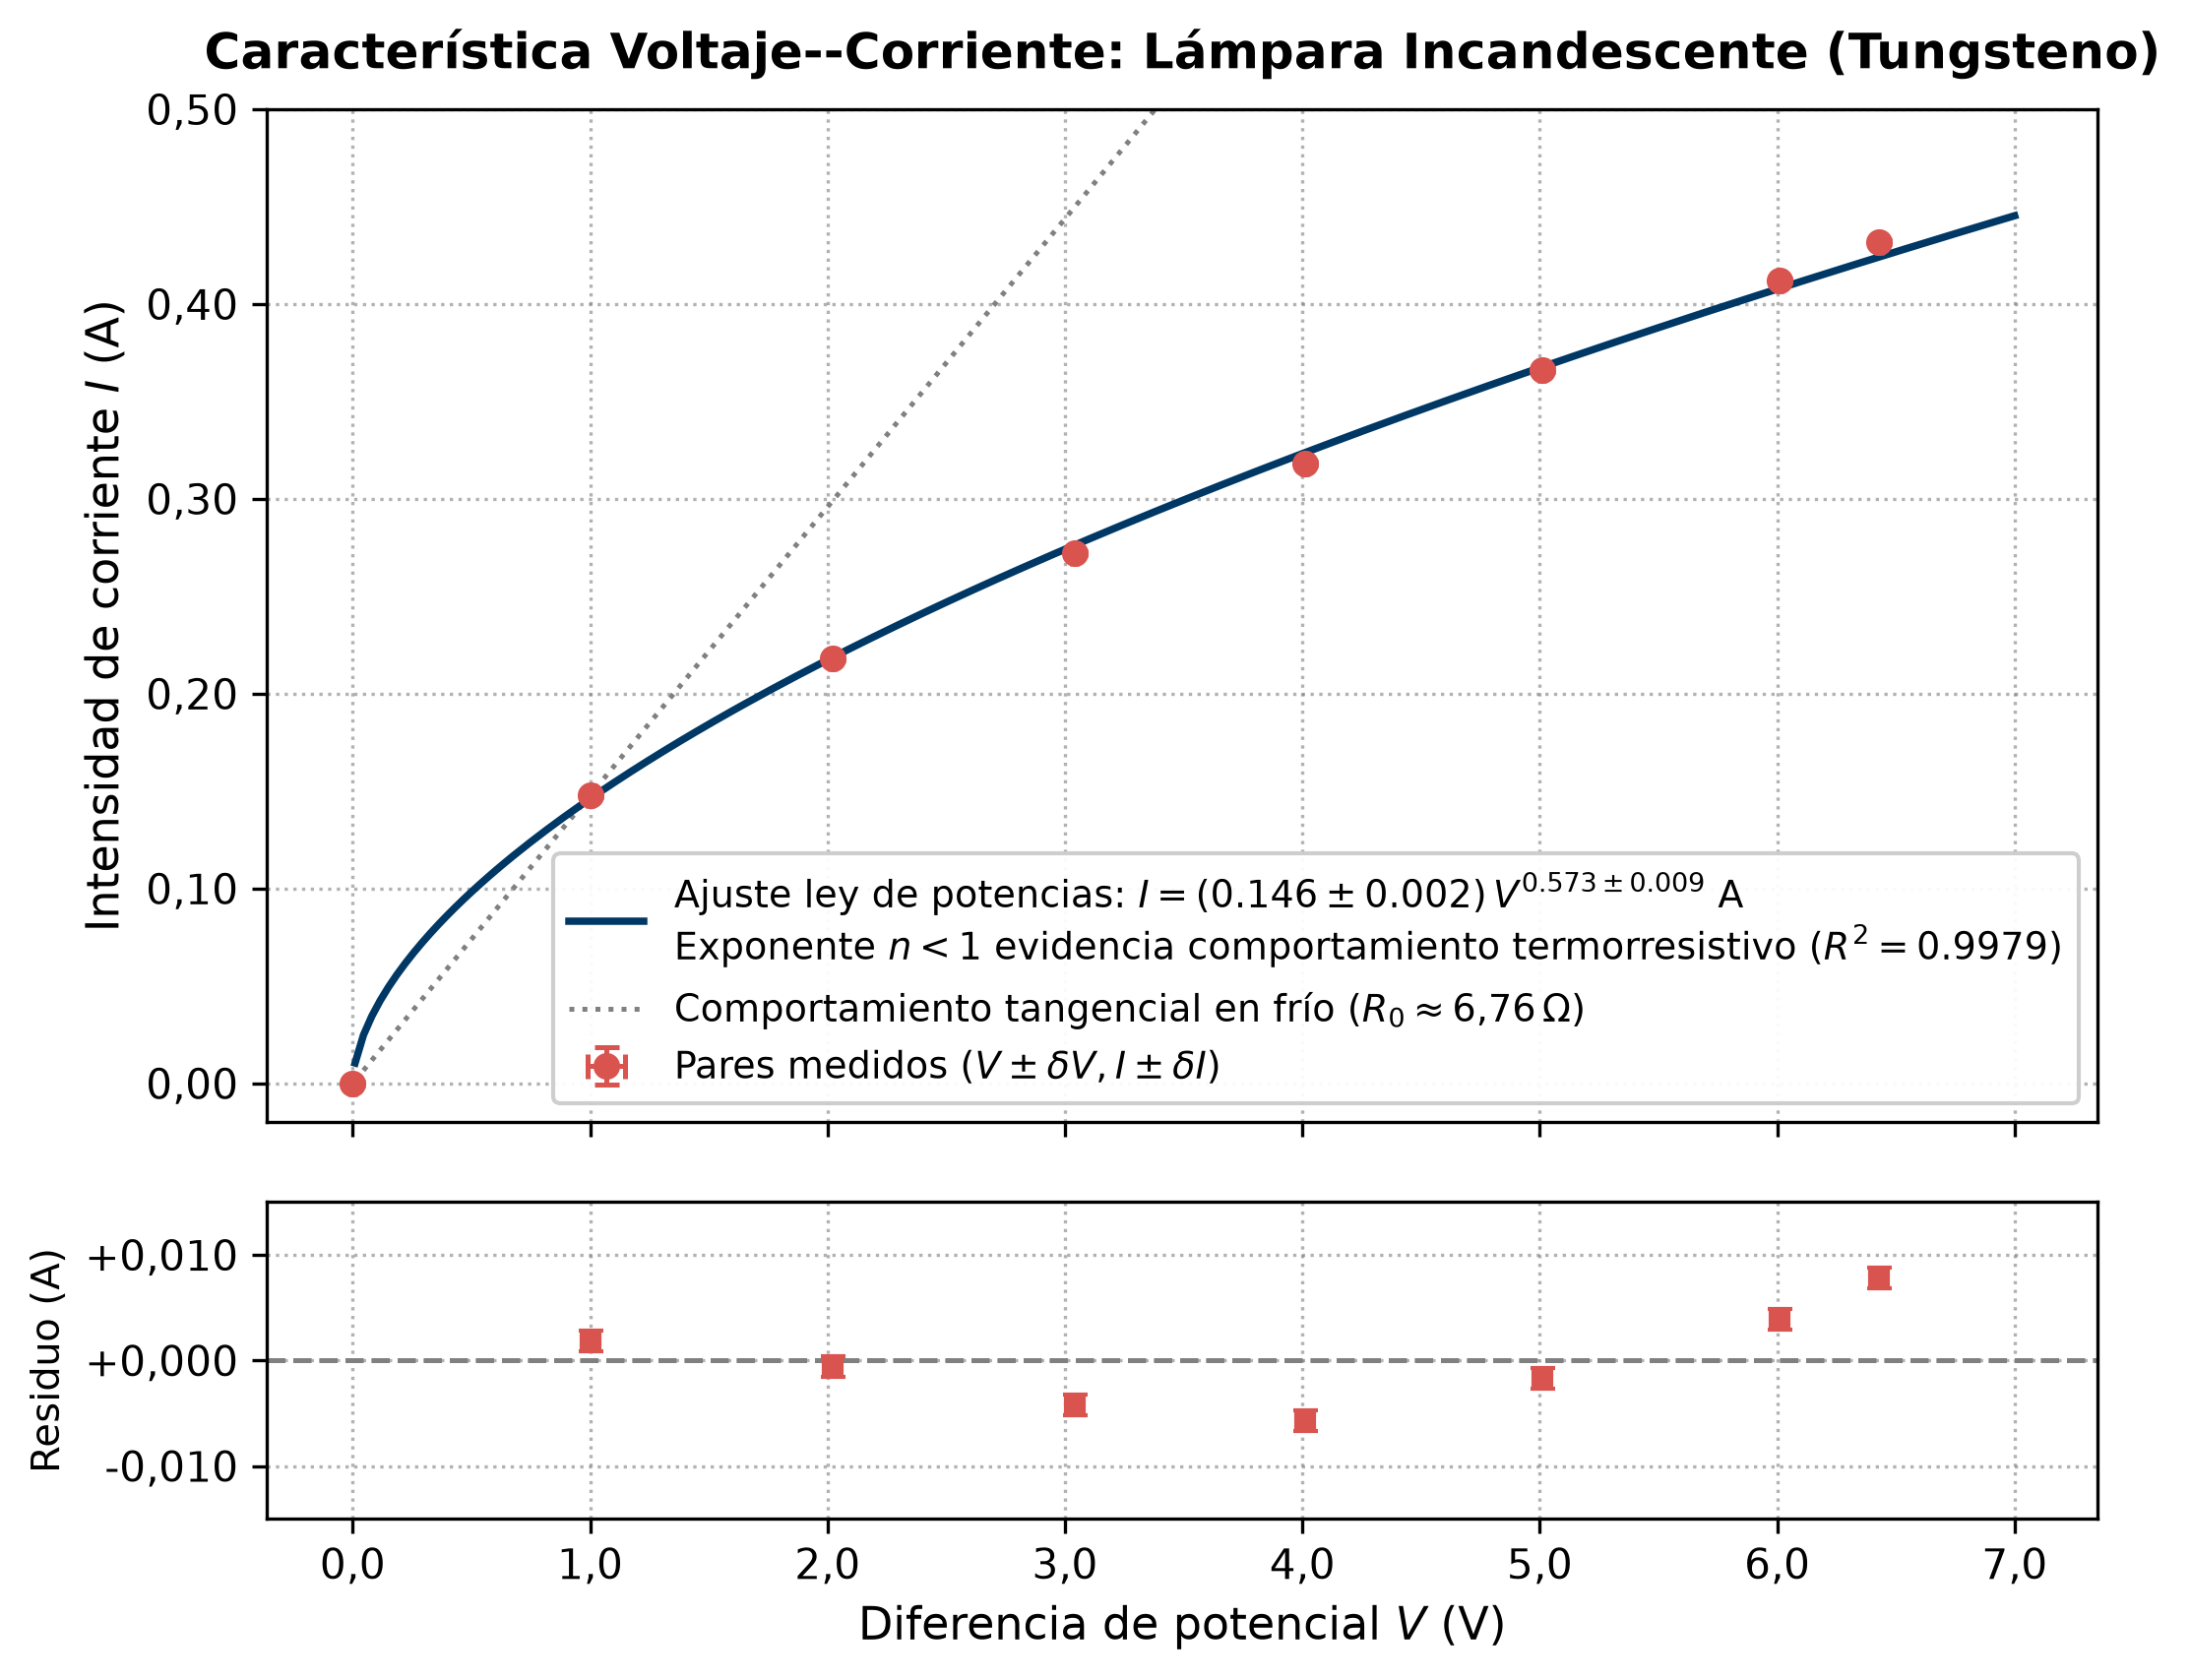
\includegraphics[width=14.0cm, height=9.0cm, keepaspectratio=true]{fig_foquito_tungsteno.png}%
}

\newpage

%% ============================================================
%% PÁGINA 4: PIERO SÁNCHEZ (GRÁFICAS CIENTÍFICAS PYTHON 3 Y 4)
%% ============================================================
\noindent
\begin{minipage}{\linewidth}
    \centering
    {\large\bfseries\color{uni-blue} GUÍA DE FIGURAS Y GRÁFICAS PARA IMPRESIÓN (STICKERS / RECORTES)}\\[0.5mm]
    {\footnotesize\textbf{Página 4 de 5: Sección 10 --- Diodo de Silicio y Comparativa Global (Piero Sánchez)}}\\[0.8mm]
    \hrule height 0.8pt
\end{minipage}

\vspace{3mm}

\stickersingle{Figura 9: Curva Característica $I$ vs $V$ del Diodo de Silicio y Tensión de Umbral ($V_u$)}{%
    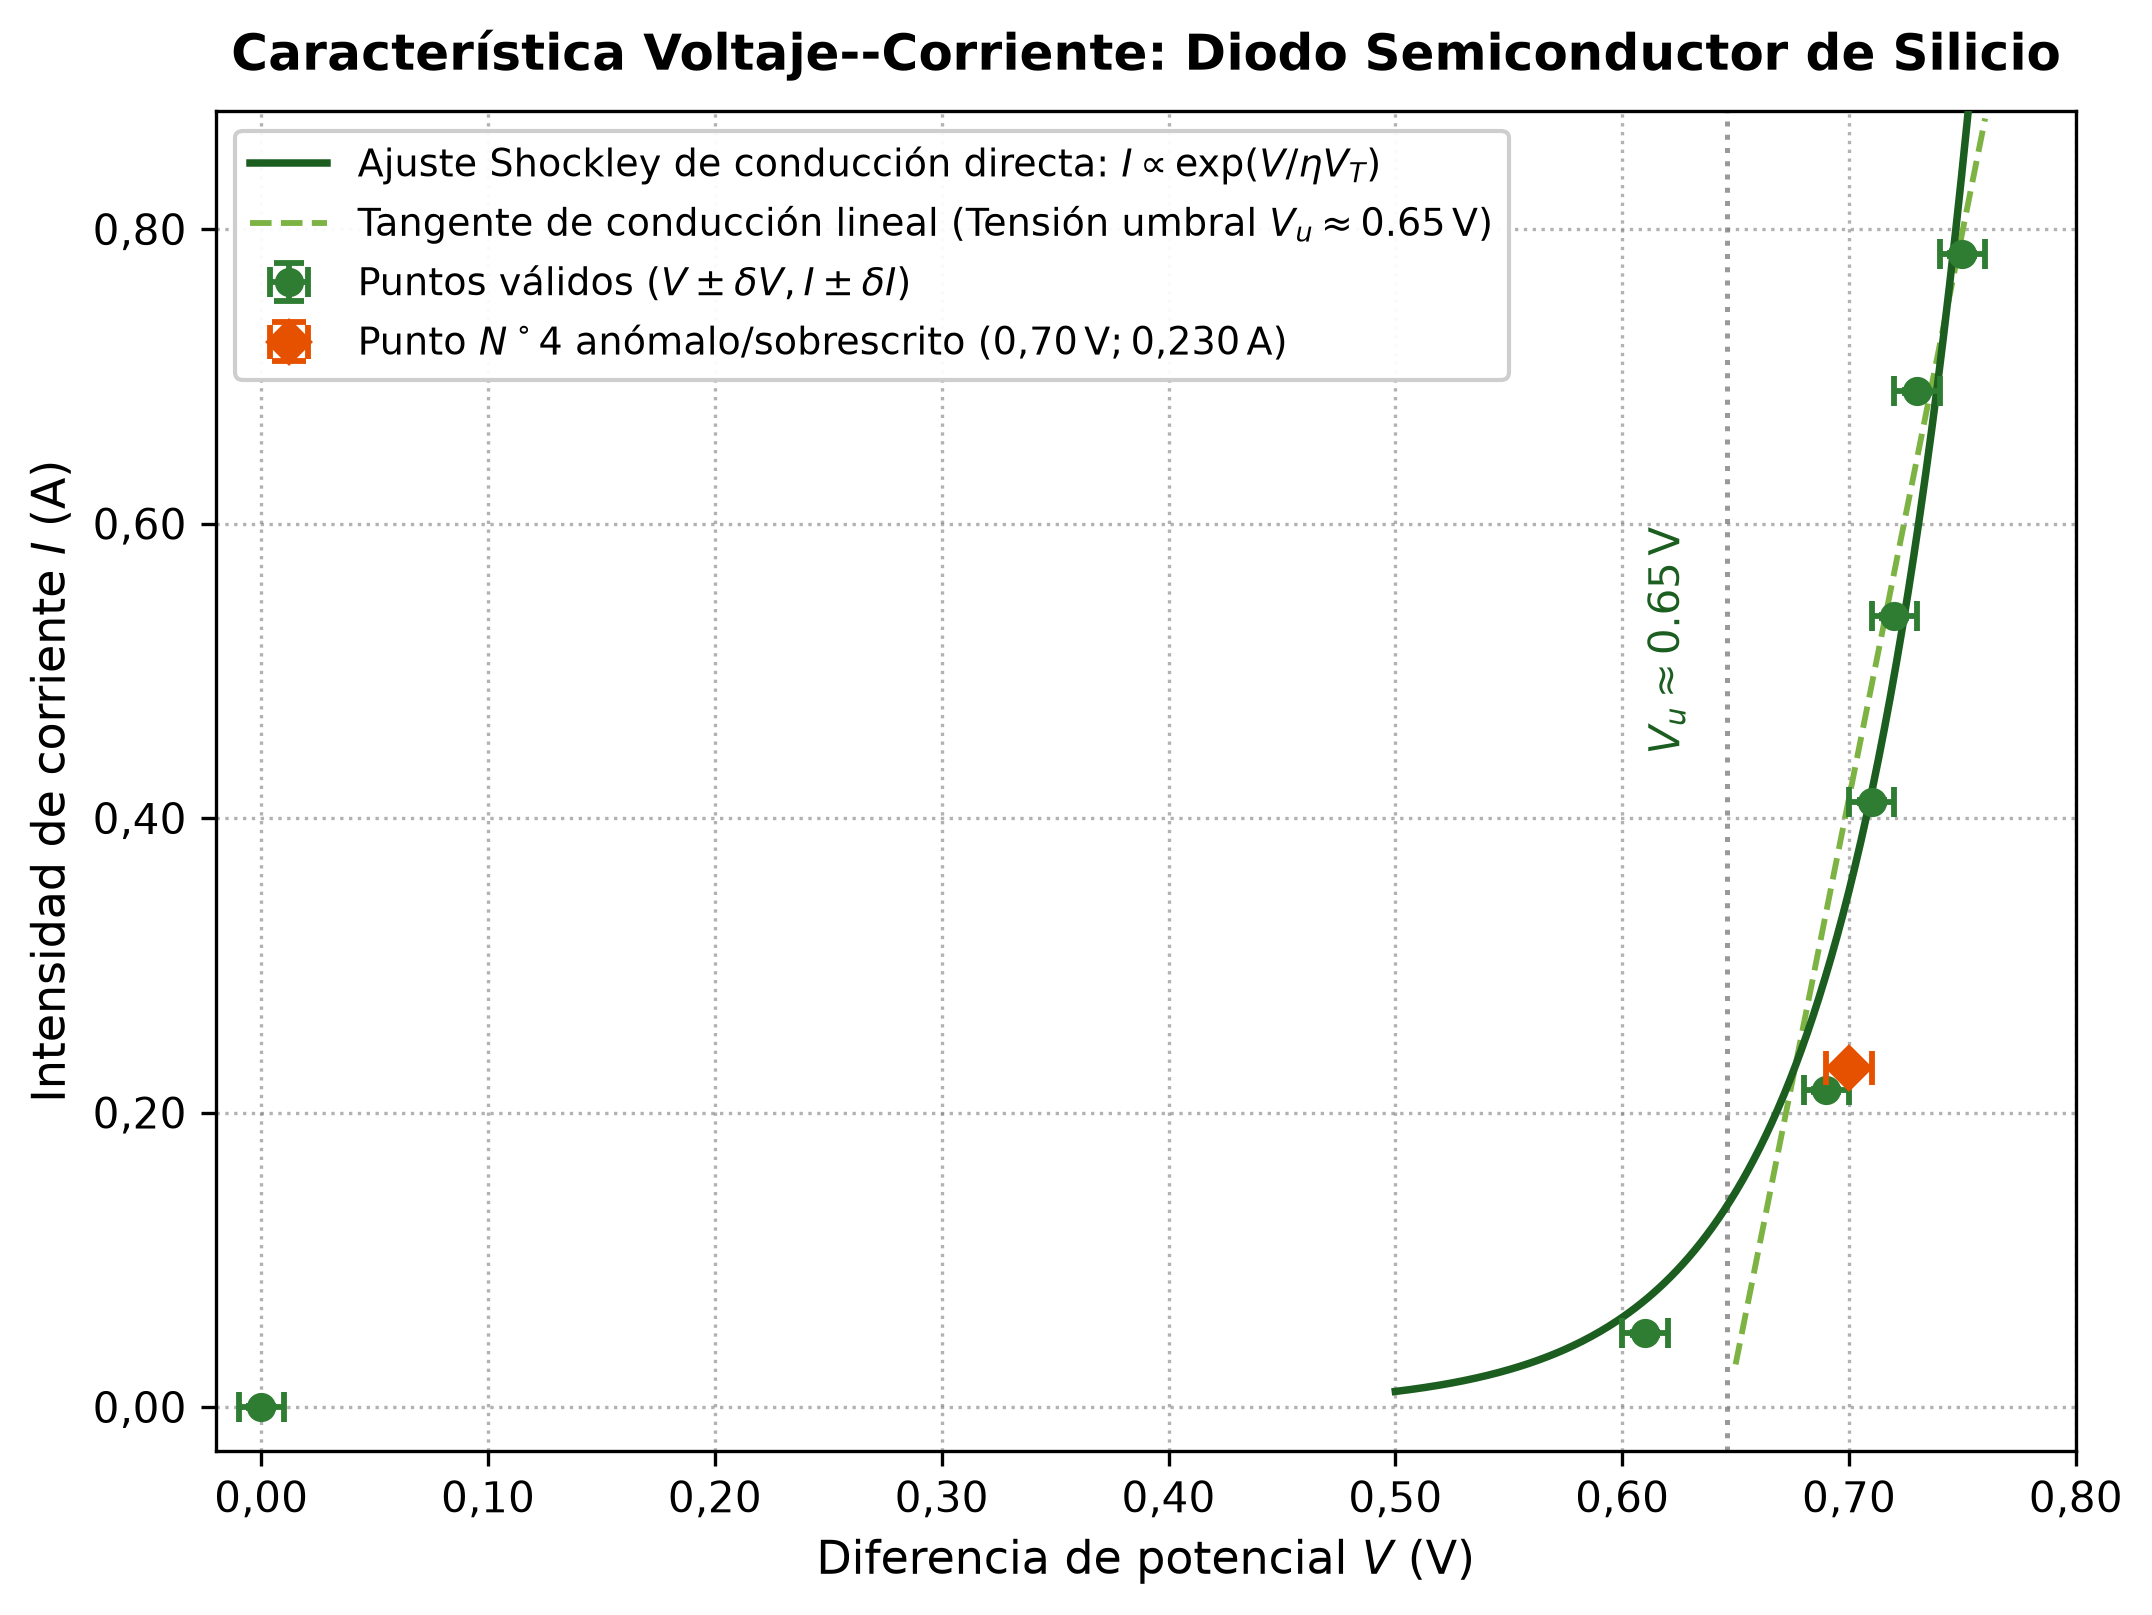
\includegraphics[width=14.0cm, height=9.0cm, keepaspectratio=true]{fig_diodo_silicio.png}%
}

\vspace{4mm}

\stickersingle{Figura 10: Contraste Comparativo Global de los Tres Elementos en Escala Común}{%
    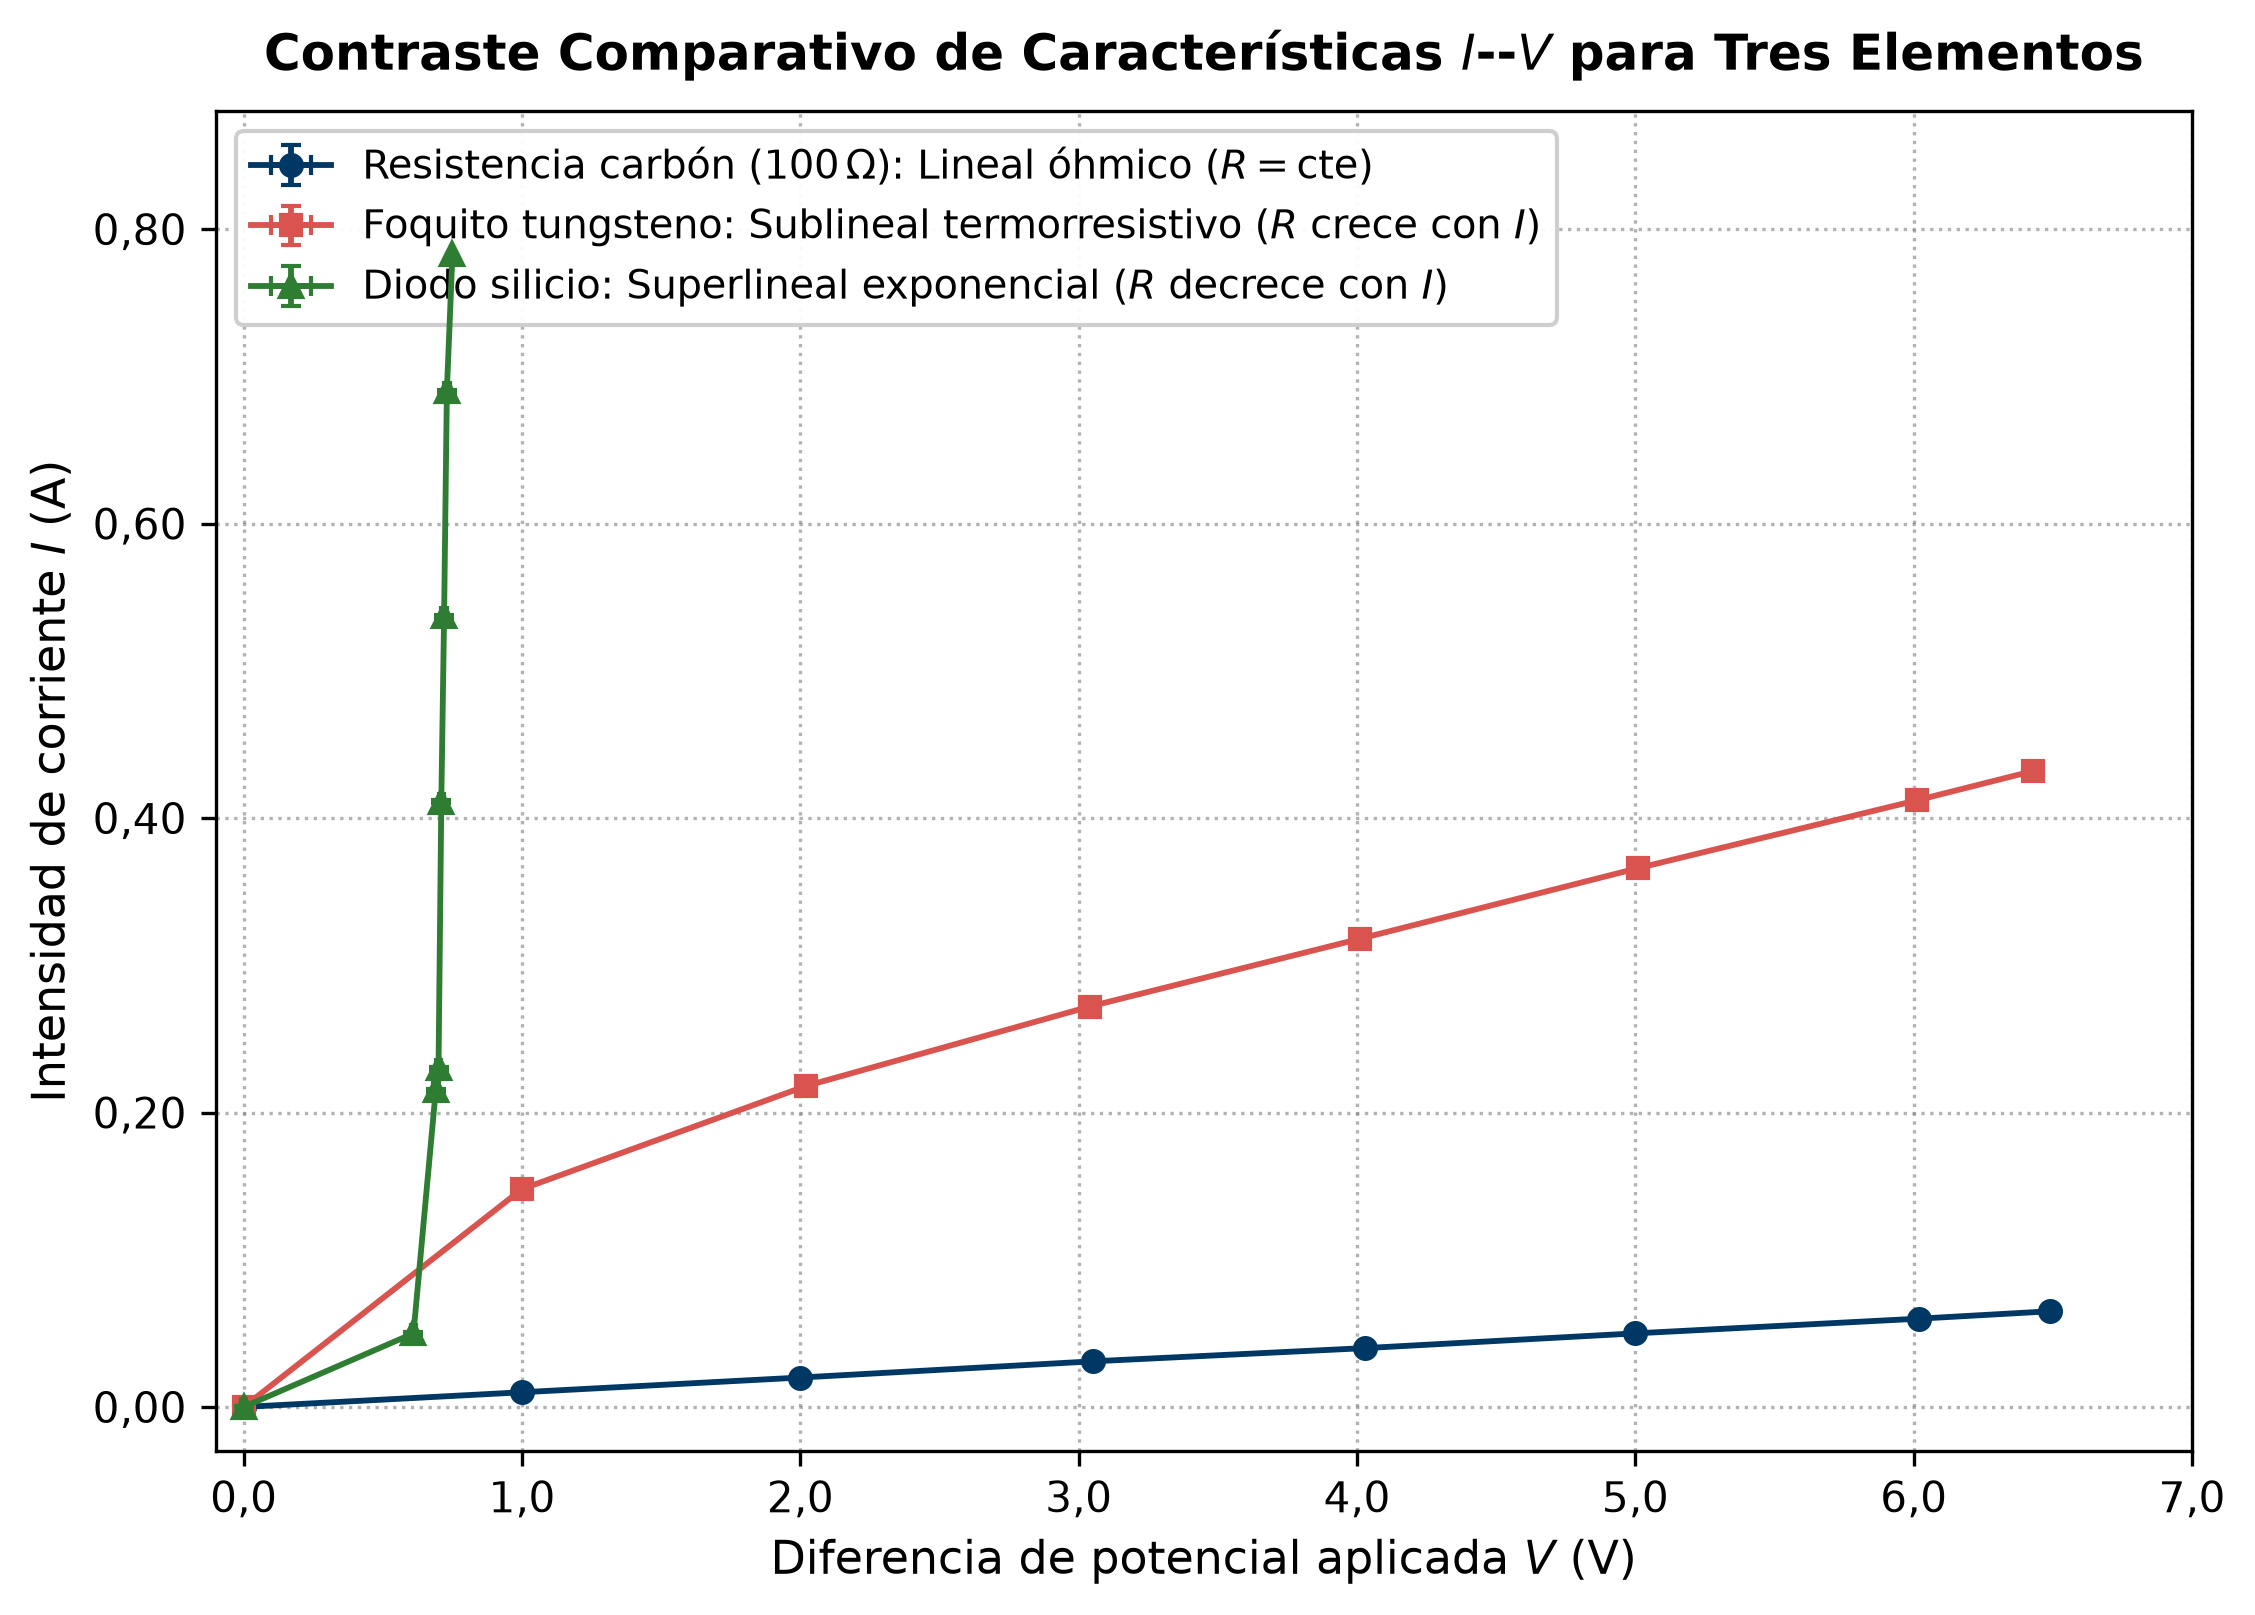
\includegraphics[width=14.0cm, height=9.0cm, keepaspectratio=true]{fig_comparativa_elementos.png}%
}

\newpage

%% ============================================================
%% PÁGINA 5: PIERO SÁNCHEZ (RESISTENCIA VS CORRIENTE Y HOJA FIRMADA)
%% ============================================================
\noindent
\begin{minipage}{\linewidth}
    \centering
    {\large\bfseries\color{uni-blue} GUÍA DE FIGURAS Y GRÁFICAS PARA IMPRESIÓN (STICKERS / RECORTES)}\\[0.5mm]
    {\footnotesize\textbf{Página 5 de 5: Sección 11 y Anexo D --- Resistencia vs Corriente y Hoja Original (Piero Sánchez)}}\\[0.8mm]
    \hrule height 0.8pt
\end{minipage}

\vspace{3mm}

\stickersingle{Figura 11: Evolución de la Resistencia Estática Aparente $R(I) = V/I$ vs Corriente}{%
    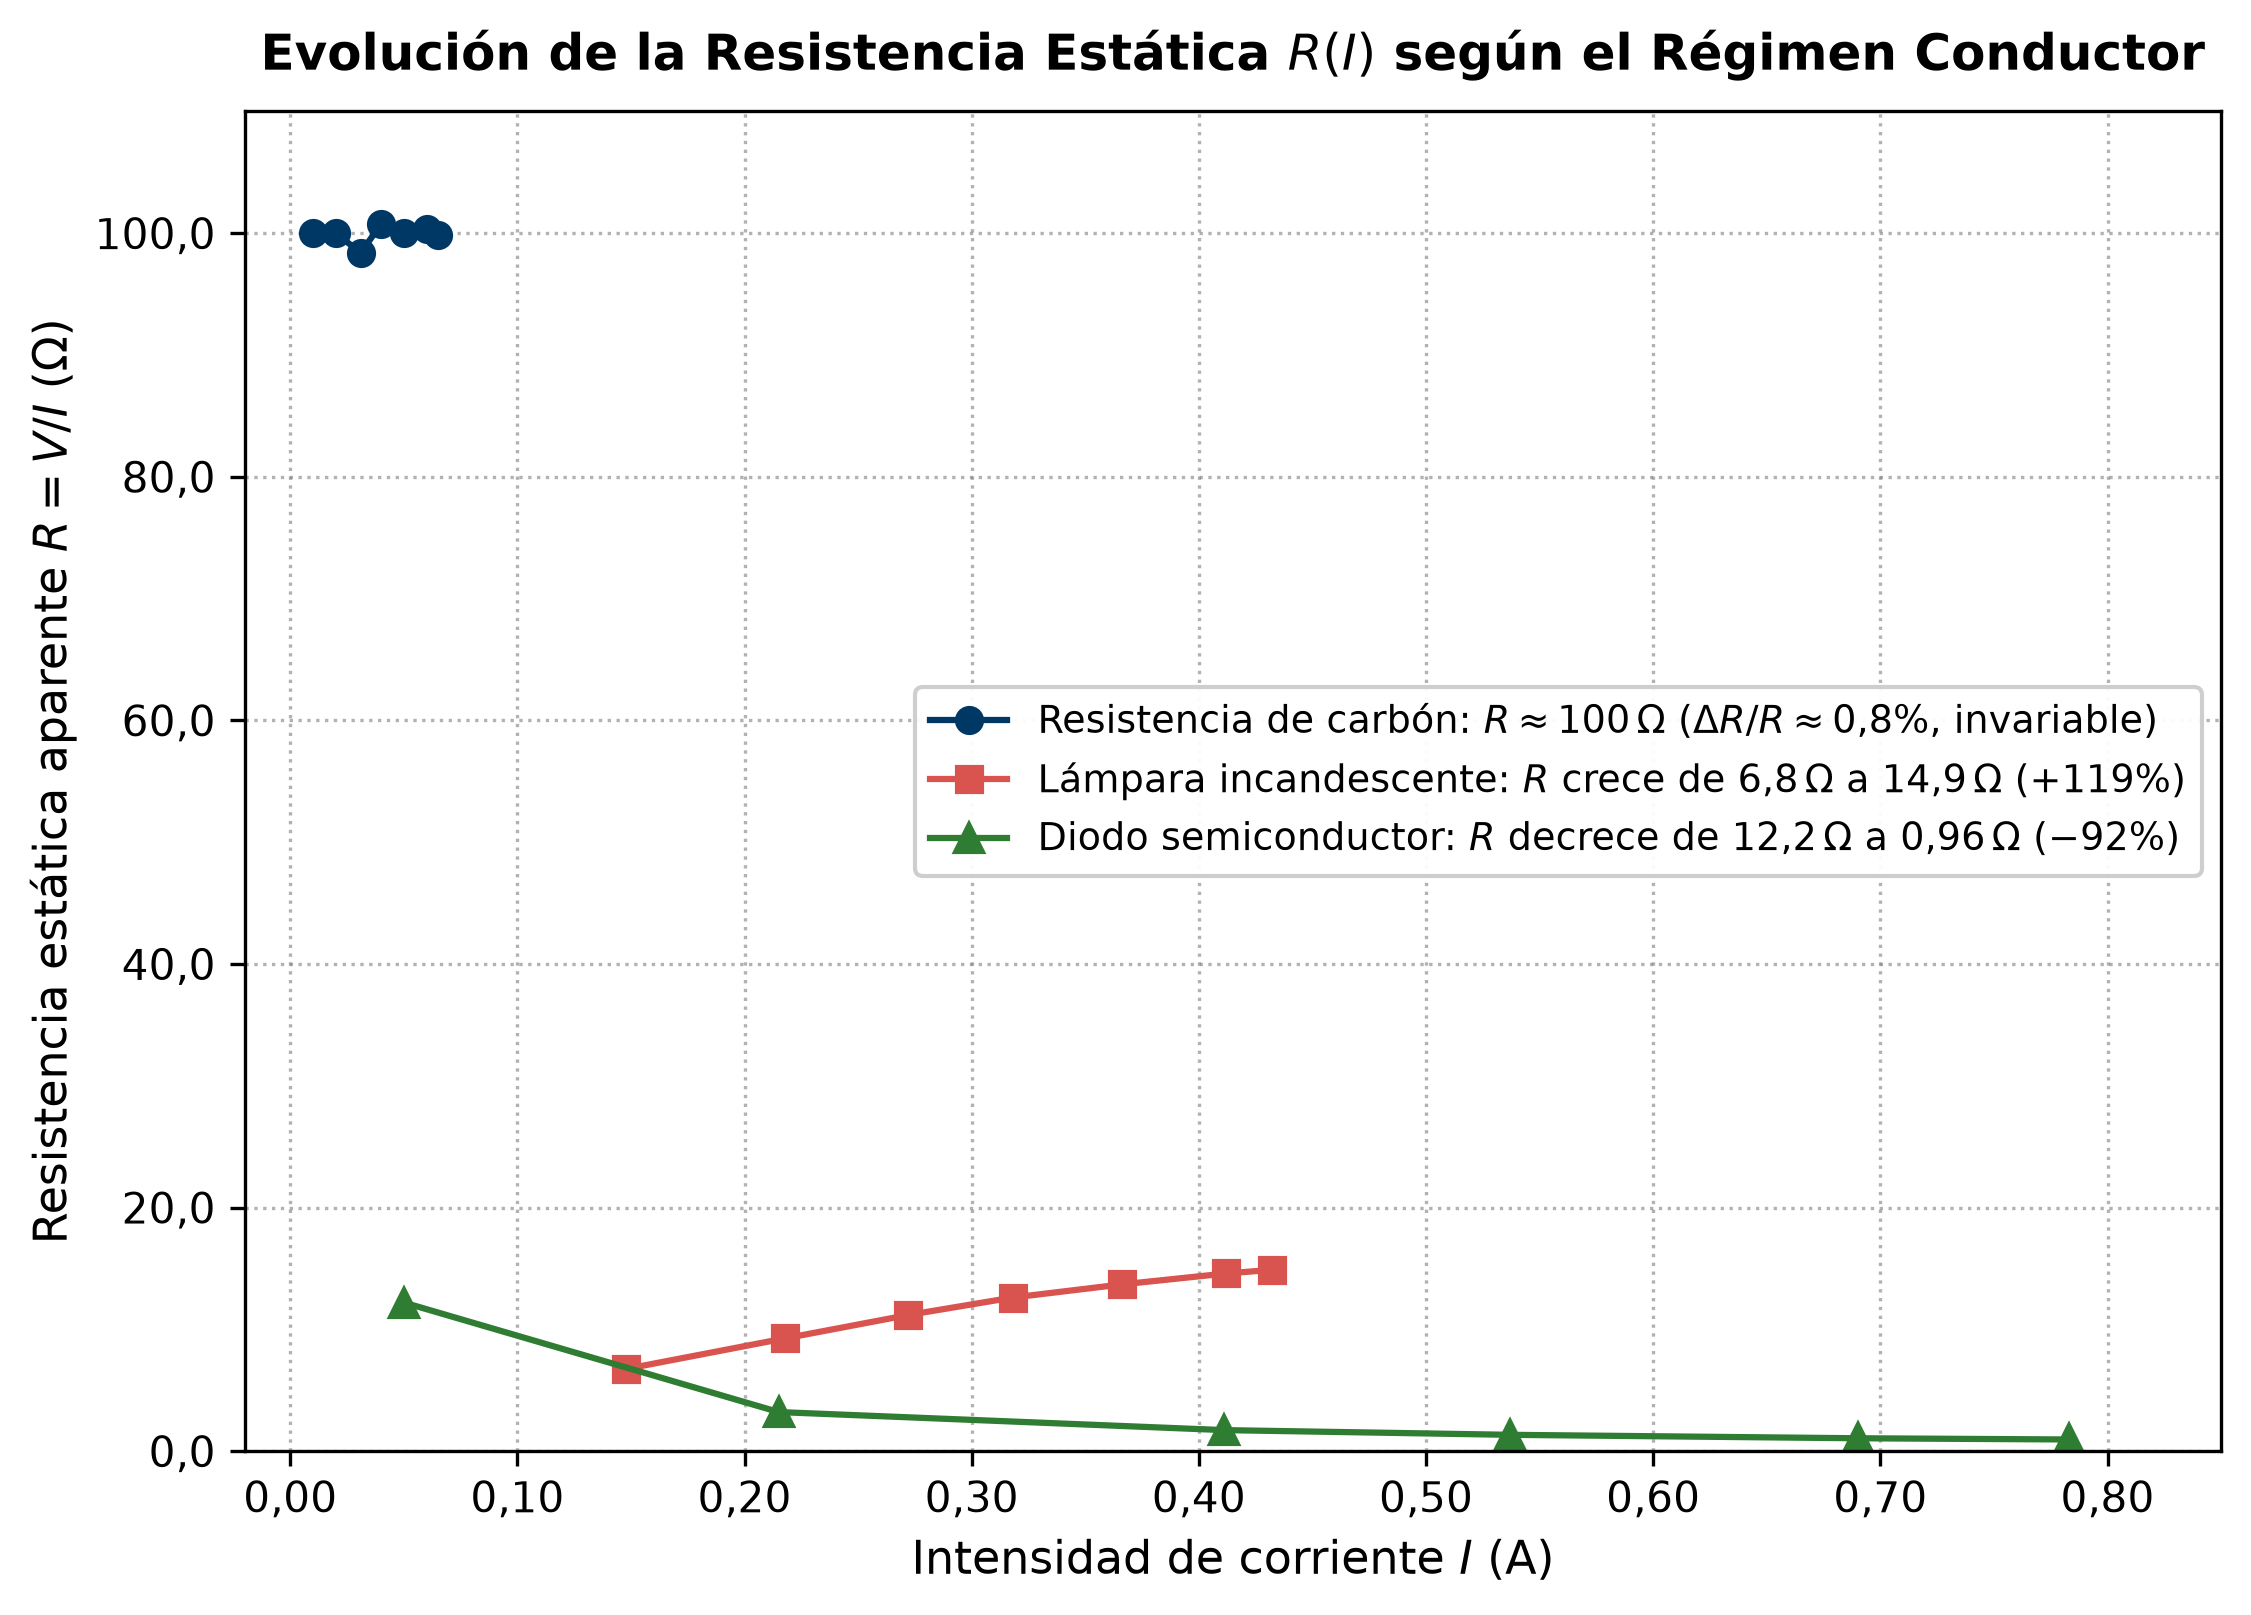
\includegraphics[width=13.5cm, height=8.2cm, keepaspectratio=true]{fig_resistencia_vs_corriente.png}%
}

\vspace{3mm}

\stickersingle{Figura 12: Facsímil de la Hoja de Datos Crudos Original Firmada en Mesa de Trabajo}{%
    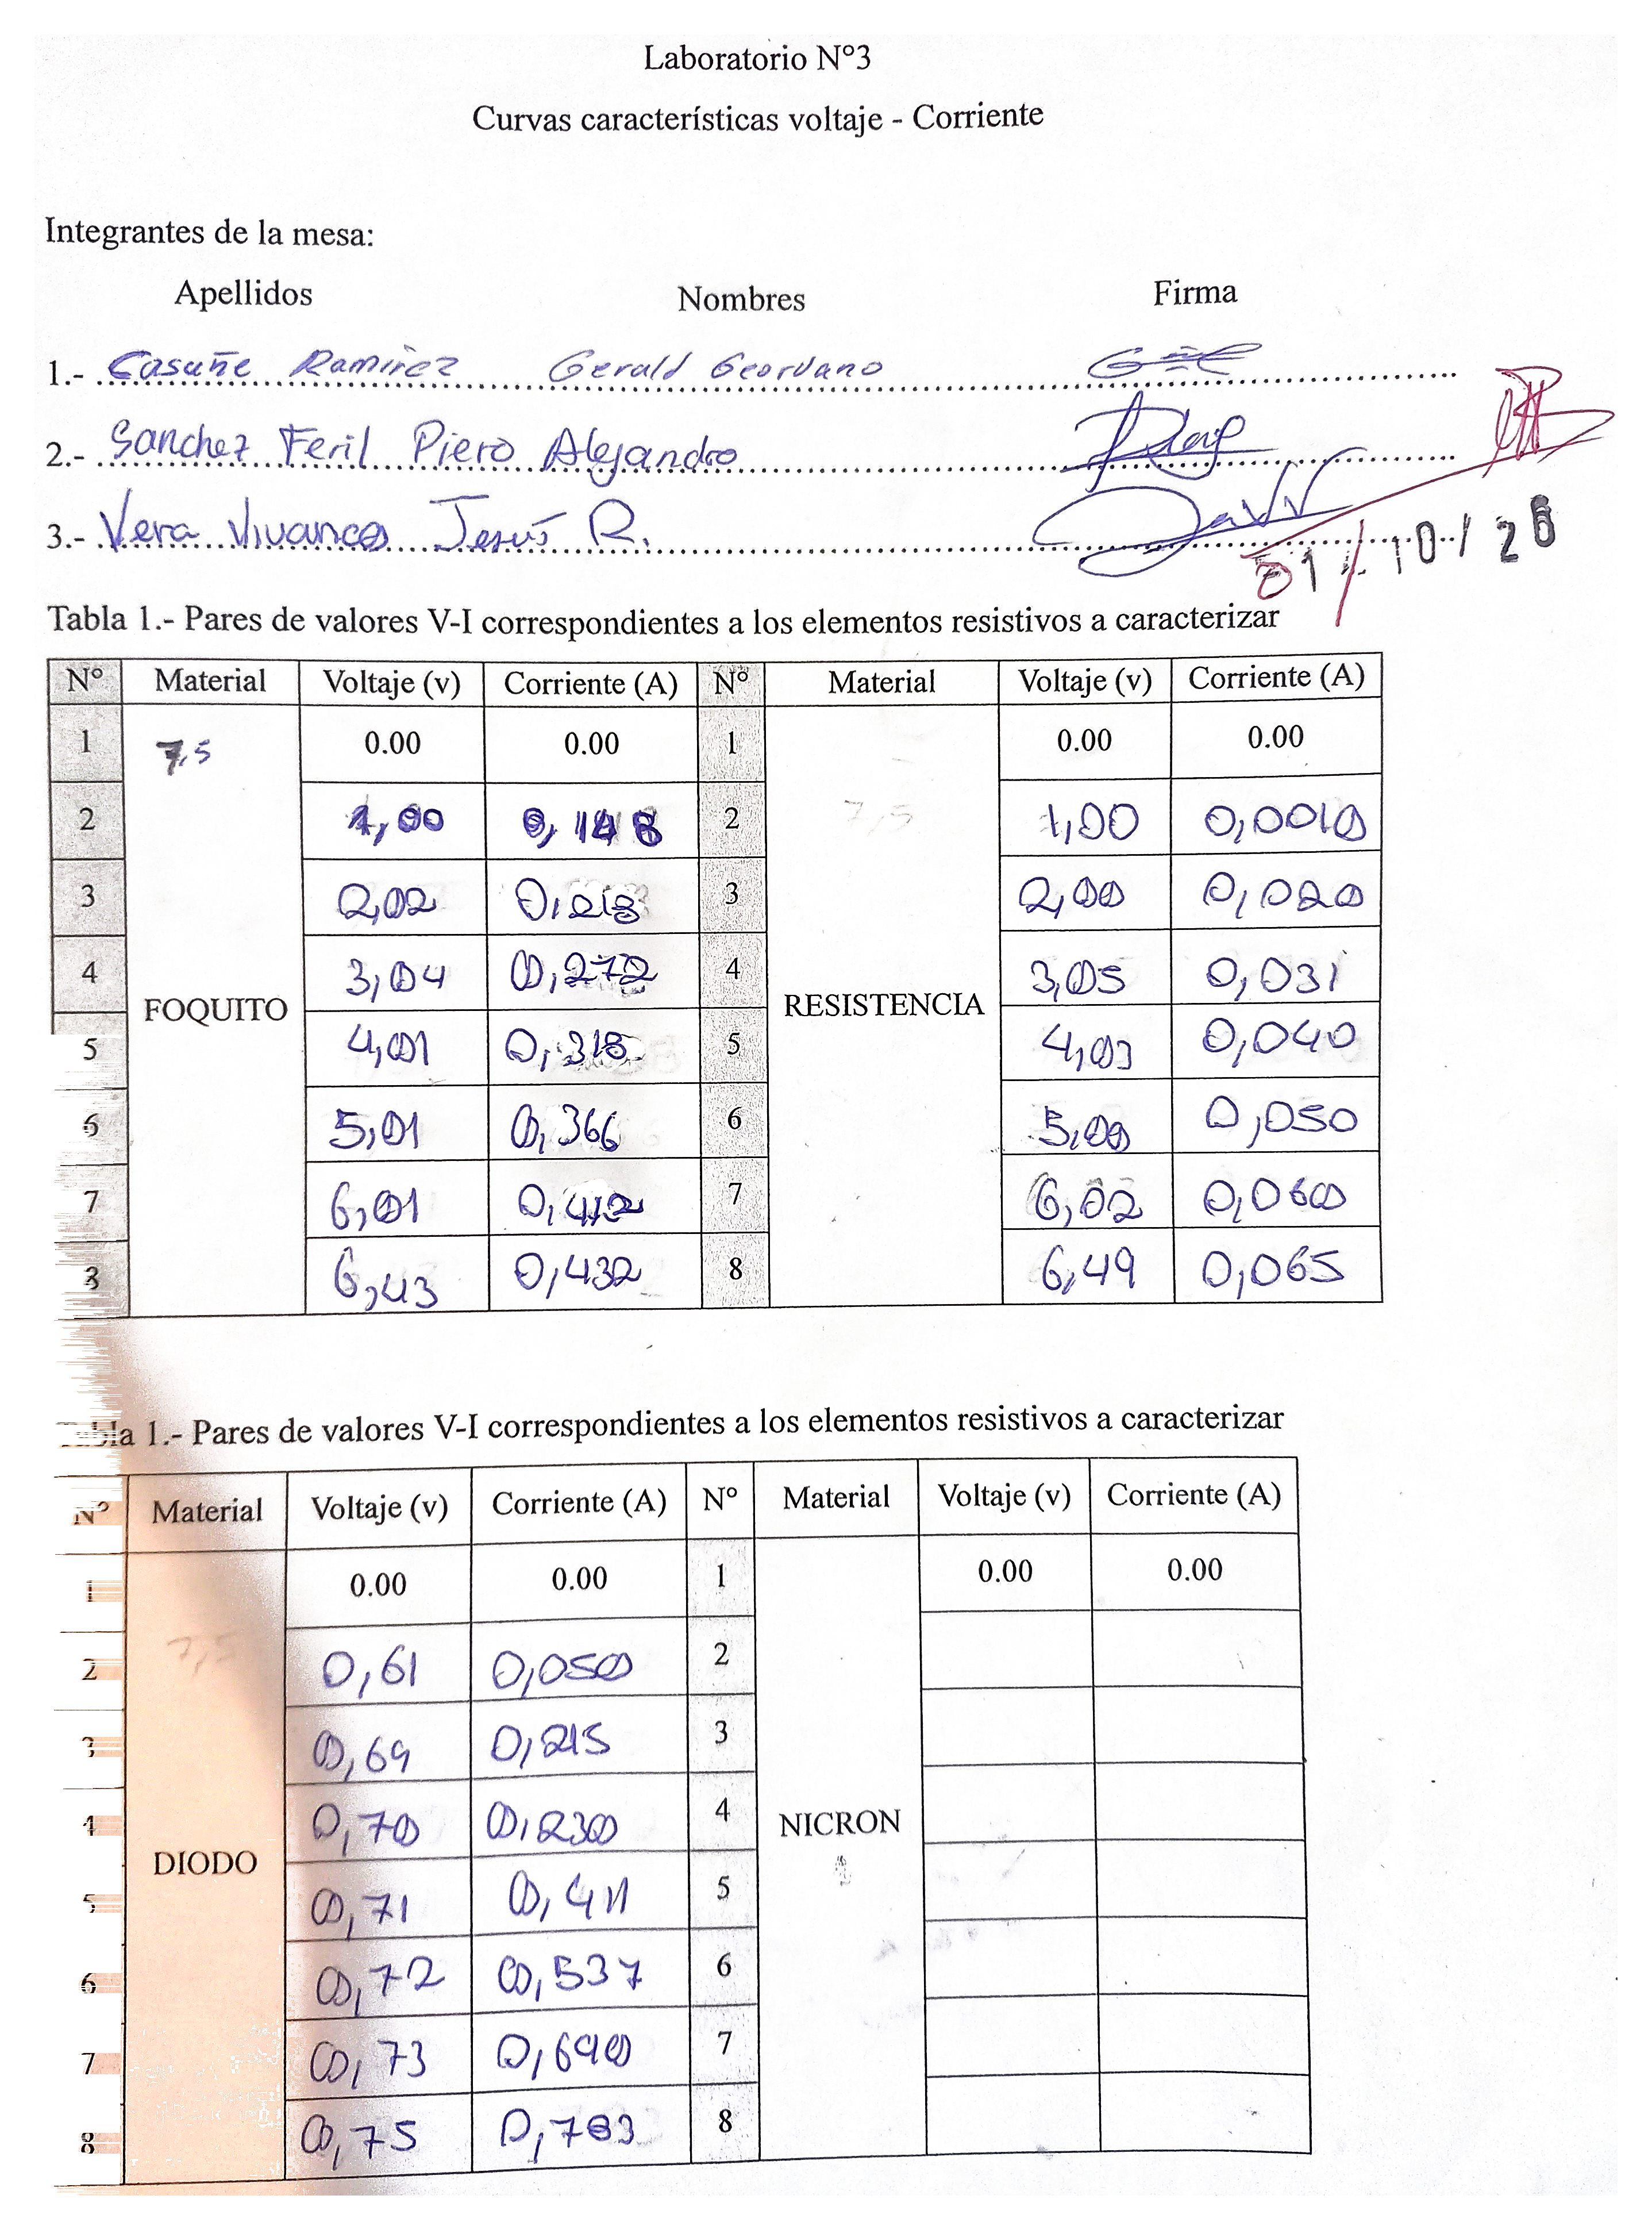
\includegraphics[width=13.0cm, height=11.5cm, keepaspectratio=true]{fig_hoja_datos.png}%
}

\end{document}
